\documentclass[conference]{IEEEtran}
\IEEEoverridecommandlockouts
\usepackage{cite}
\usepackage{amsmath,amssymb,amsfonts}
\usepackage{algorithm}
\usepackage{algpseudocode}
\usepackage{graphicx}
\usepackage{textcomp}
\usepackage{xcolor}
\usepackage{booktabs}
\usepackage{url}
\usepackage{pifont}
\newcommand{\cmark}{\ding{51}}
\newcommand{\xmark}{\ding{55}}

\def\BibTeX{{\rm B\kern-.05em{\sc i\kern-.025em b}\kern-.08em
    T\kern-.1667em\lower.7ex\hbox{E}\kern-.125emX}}

\begin{document}

\title{Adaptive Session Resumption for Hybrid Post-Quantum Authentication\\ in Wearable Healthcare IoT}

\author{
\IEEEauthorblockN{Manjith Mugundan T A}
\IEEEauthorblockA{Dept. of Computer Science and Engineering\\
Karunya Institute of Technology and Sciences\\
Coimbatore, India\\
manjithmugundan@karunya.edu.in}
\and
\IEEEauthorblockN{Priscilla Joy R}
\IEEEauthorblockA{Dept. of Computer Science and Engineering\\
Karunya Institute of Technology and Sciences\\
Coimbatore, India\\
priscillajoy@karunya.edu}
}

\maketitle

\begin{abstract}
Wearable healthcare devices continuously exchange sensitive medical data over
wireless networks, making secure authentication essential. This paper
retains the classical Ed25519 signature only for lightweight device identity
verification, while ML-KEM-512 (FIPS 203) supplies the quantum-resistant
guarantee for session-key establishment; repeating this full hybrid
handshake on every reconnection of a resource-constrained device is
nonetheless too costly. The central contribution is an Adaptive Session
Security Manager (SSM) that decides, per reconnection, whether a full
Ed25519 + ML-KEM-512 handshake or a bounded, HMAC-protected lightweight
resumption applies, governed by session lifetime, resumption count, and a
formalized anomaly-scoring algorithm whose threshold is set so that the
anomaly branch is mathematically reachable within the score's own declared
range -- correcting an inconsistency identified during this project's own
reproducibility audit of an earlier version of this work. Every performance
figure reported here is measured, not cited or assumed: we built an
open-source reference implementation of the full protocol (real Ed25519,
ML-KEM-512, HMAC-SHA256, AES-128-GCM and HKDF) and benchmarked every
operation directly on commodity hardware, then ran the SSM's decision logic
event-by-event over accelerometer telemetry from 97 real subject-sessions of
a real Bluetooth-connected wearable (the PhysioNet Empatica E4
wearable-device dataset), explicitly preserving three real, documented
Bluetooth-disconnection gaps in the session timeline rather than
concatenating them away, and explicitly documenting a signal-duplication
truncation applied to one subject's recording. This trace-driven evaluation
shows the proposed framework reduces authentication compute time by
83.7--87.3\% and transmitted bytes by 75.3--78.6\% relative to an
always-full hybrid baseline, depending on activity regime. The protocol was
verified in ProVerif for a single session, with all eight secrecy and
injective-correspondence queries verified true; an unbounded/replicated
verification attempt is also reported, honestly, as producing one
unresolved finding that is most likely a modeling limitation rather than a
confirmed protocol flaw. A comparison against recent hybrid post-quantum
healthcare-IoT proposals suggests that, to the best of our knowledge, this
adaptive-resumption gap is not addressed elsewhere in the surveyed
literature.
\end{abstract}

\begin{IEEEkeywords}
post-quantum cryptography, ML-KEM, Ed25519, session resumption, wearable healthcare, adaptive authentication, IoMT
\end{IEEEkeywords}

\section{Introduction}

Wearable healthcare IoT devices continuously monitor physiological
parameters and relay this data through a gateway to cloud healthcare
servers. Medical data is sensitive, regulated, and long-lived, so any
compromise has lasting consequences. Most deployed systems still rely on
classical cryptography (RSA, ECC), which is efficient but provably breakable
by Shor's algorithm once sufficiently capable quantum computers exist,
exposing captured traffic to ``harvest now, decrypt later'' attacks
\cite{shor1994}. NIST-standardized ML-KEM (CRYSTALS-Kyber) \cite{fips203}
addresses this, but its larger keys and heavier computation are difficult to
justify if a full handshake repeats on every connection.

Existing hybrid classical/PQC proposals reduce this burden by combining a
lightweight classical signature with a PQC key exchange, but they still
perform the full handshake on every reconnection, regardless of how recently
the device last authenticated. Wearable devices reconnect far more often
than this assumption allows due to Bluetooth Low Energy (BLE) range loss and
duty-cycled sleep. This paper introduces a Session Security Manager (SSM) --
a bounded decision layer backed by a formalized anomaly-scoring algorithm --
that governs when a full Ed25519 + ML-KEM-512 handshake is necessary and
when a lightweight HMAC resumption suffices, without weakening
quantum-resistance guarantees.

\subsection{Contributions}

(1) An adaptive hybrid framework combining Ed25519 identity verification
with ML-KEM-512 quantum-resistant key establishment for lightweight wearable
authentication. (2) A novel SSM (Algorithm~1) governed by a formalized
Anomaly Scoring Algorithm (Algorithm~2), whose threshold is set so that its
own decision branch is mathematically reachable within the score's declared
range -- a correction made explicit and pre-registered before any
experiment reported here was run, in response to an inconsistency this
project's own reproducibility investigation found in an earlier iteration
of this design. (3) A fully reproducible, trace-driven evaluation
methodology: an open-source cryptographic reference implementation
benchmarked directly rather than cited from the literature, combined with
real accelerometer telemetry and three documented Bluetooth-disconnection
events from a public wearable-device dataset, with an explicit,
pre-registered methodology for how split recordings and a documented
signal-duplication are handled. (4) A threat model, protocol-level security
analysis, and a structural formal-verification model, including an honest
report of an unresolved finding from an unbounded verification attempt.

\section{Related Work and Research Gap}

Authentication for wearable healthcare systems has traditionally relied on
RSA- or ECC-based cryptography because of low computational cost and mature
implementations. These schemes remain efficient on existing hardware but
offer no protection against quantum adversaries, motivating adoption of
post-quantum cryptographic (PQC) algorithms for long-term healthcare data
protection \cite{fips203,shor1994}. As NIST-standardized PQC algorithms have
matured, several works have evaluated their embedded performance: ML-KEM/Kyber
shows strong results on ARM Cortex-M4 microcontrollers \cite{pqm4}, while
Dilithium-family signatures raise memory and packet-fragmentation concerns
on constrained radios such as BLE.

Hybrid classical/PQC designs, recommended as a gradual transition strategy,
combine a lightweight classical signature with a PQC key exchange to
balance security and cost. Several recent works apply this specifically to
medical/wearable IoT \cite{abood2025,adeli2023,alsaggaf2022,yan2026}:
fog-assisted PQC key-encapsulation schemes for IoHT, PQC-compliant
authentication for IoT healthcare systems, a two-factor fuzzy-commitment
authentication protocol with a random-oracle-model proof for IoT-enabled
healthcare, and a Kyber-based cloud-assisted authentication scheme for
medical IoT. These establish that hybrid PQC authentication for medical IoT
is an active, competitive research area, and that formal or ROM-style
proofs are increasingly an expected component rather than an optional
addition.

However, across all surveyed works, the handshake structure is uniform: a
full authentication and key-exchange sequence runs at every connection
event, irrespective of how recently the device last authenticated. None
introduces a mechanism to distinguish a first-time or long-idle connection,
where a full quantum-resistant handshake is clearly warranted, from a
routine reconnection occurring minutes after the previous authenticated
session, where it may not be. Given that wearable-to-gateway links reconnect
frequently due to BLE range loss, interference, and duty-cycled sleep modes,
this uniform-cost assumption represents a genuine and addressable
inefficiency rather than a hypothetical one (Table~\ref{tab:related}). We
address this by separating lightweight, bounded session verification from
quantum-resistant key establishment, governed by an explicit, formalized
decision layer -- rather than proposing yet another combination of
classical and post-quantum primitives.

\begin{table}[t]
\caption{Comparison with Related Approaches}
\label{tab:related}
\centering
\resizebox{\columnwidth}{!}{%
\begin{tabular}{lcccc}
\toprule
Work & PQ key est. & Adaptive auth. & Session resume & Anomaly logic \\
\midrule
ECC-based & \xmark & \xmark & \xmark & \xmark \\
Hybrid IoT \cite{abood2025} & \cmark & \xmark & \xmark & \xmark \\
Med-Sec-IoT \cite{alsaggaf2022} & \cmark & \xmark & \cmark & \xmark \\
\textbf{Proposed} & \cmark & \cmark & \cmark & \cmark \\
\bottomrule
\end{tabular}%
}
\end{table}

\section{System Model}

The system has three entities: a resource-constrained Wearable Device (WD)
holding Ed25519 and ML-KEM-512 key pairs; a Gateway (GW) that terminates the
protocol and hosts the SSM and ticket store; and a Healthcare Server (HS)
that stores credentials and receives authenticated data. Every WD--GW
connection is mediated by the SSM before any data is forwarded.

\subsection{Threat Model}

The protocol is analyzed under the Dolev--Yao adversary: full channel
control, able to eavesdrop, intercept, delay, replay, inject, or modify
messages, but unable to break the underlying primitives or long-term
private keys directly. Key compromise is treated as an out-of-scope problem
addressed by secure storage, not by the protocol itself.

\subsection{Design Goals}

Lightweight WD computation; quantum-resistant key establishment; low
latency for real-time monitoring; low communication overhead (BLE-safe
message sizes); scalability across many devices; and bounded, secure
session reuse without repeating full-handshake cost on every reconnection.

\section{Proposed Framework}

The contribution is not the choice of Ed25519, ML-KEM-512, and AES-128-GCM
individually -- each is a standard implementation choice -- but the SSM
policy layer governing which path a reconnection takes.

\subsection{Registration and Full Authentication}

Each WD is registered with a unique identity and Ed25519 key pair
($PK_i = \mathrm{Gen}(SK_i)$). Ed25519 is used specifically because it
produces a compact 64-byte signature with fast verification and low memory
footprint, unlike RSA (large keys) or Dilithium-family PQC signatures
($\approx$2.4~KB, risking BLE packet fragmentation). On first connection:

\begin{enumerate}
\item WD$\to$GW: connect request
\item GW$\to$WD: nonce $N_1$
\item WD signs $N_1$ ($\sigma_1$), sends $\{\sigma_1, N_2\}$
\item GW verifies $\sigma_1$
\item GW performs ML-KEM-512 encapsulation, producing ciphertext $ct$
\item GW signs $N_2$ jointly with $ct$ ($\sigma_2 = \mathrm{Sign}(N_2 \| ct)$) and sends $\{\sigma_2, ct\}$
\item WD verifies $\sigma_2$ against $(N_2, ct)$ -- mutual auth complete -- then decapsulates $ct$ to recover shared secret $SS$
\end{enumerate}

Binding $ct$ into $\sigma_2$ rather than signing $N_2$ alone is a
deliberate design choice, not a stylistic one: this project's formal
verification (Sec.~\ref{sec:fv}) confirms that signing $N_2$ alone would
allow an attacker to substitute their own ML-KEM ciphertext -- encrypted
under WD's genuine public key, which is not secret -- causing WD to derive
a session key the attacker already knows. Binding $ct$ into the signature
closes this gap, and the reference implementation enforces it
(\texttt{src/protocol/protocol.py}: \texttt{sigma2 = self.ed\_sk.sign(n2 + ct)}).
ML-KEM-512 is used because it is the NIST-standardized (FIPS 203) KEM, its
security rests on Module-LWE -- not known to be efficiently solvable by
quantum algorithms -- and it offers a favorable size/cost balance among
standardized PQC options. Both parties derive:

\begin{equation}
\begin{aligned}
K_s &= \mathrm{HKDF}(SS, N_1, N_2), \\
K_r &= \mathrm{HKDF}(SS, \text{``resumption''}, N_1, N_2)
\end{aligned}
\label{eq:kdf-full}
\end{equation}

The GW issues ticket $T = \mathrm{Enc}_{K_r}(ID, \mathit{expiry}, \mathit{count}{=}0)$;
the session begins with $K_s$.

\subsection{Lightweight Resumption}

WD presents $\{T, N_3\}$; GW returns $\mathit{tag}_1 = \mathrm{HMAC}_{K_r}(N_3 \| \mathit{count})$;
WD verifies and returns $\mathit{tag}_2 = \mathrm{HMAC}_{K_r}(N_4 \| \mathit{count}{+}1)$;
GW verifies -- no ML-KEM or Ed25519 operation is performed.

\begin{equation}
K_s' = \mathrm{HKDF}(K_r, N_3, N_4, \mathit{count})
\label{eq:kdf-resume}
\end{equation}

The reference implementation (\texttt{src/protocol/protocol.py}) gates
progress on this verification strictly: a failed tag check raises before
any counter or state update occurs, and the shared \texttt{count} is
advanced only after the check succeeds, closing a premature-acceptance
class of flaw this project's formal model checks for explicitly
(Sec.~\ref{sec:fv}).

\subsection{Algorithm 1 --- SSM Decision Logic}
\label{sec:alg1}

\begin{algorithm}[t]
\caption{SSM Decision Logic}
\label{alg:ssm}
\begin{algorithmic}[1]
\Require elapsed, resumption\_count, score $S$ (Alg.~2), has\_prior\_ticket
\If{\textbf{not} has\_prior\_ticket}
  \State \Return FULL\_AUTH \Comment{Rule 0: explicit first-session case}
\ElsIf{elapsed $>$ $T_{max}$}
  \State \Return FULL\_AUTH
\ElsIf{resumption\_count $\geq$ $R_{max}$}
  \State \Return FULL\_AUTH
\ElsIf{$S \geq A_{th}$}
  \State \Return FULL\_AUTH
\Else
  \State \Return RESUME
\EndIf
\end{algorithmic}
\end{algorithm}

Line~1--2 (``Rule~0'') is an explicit, documented addition over earlier
iterations of this design: the very first connection from a device with no
prior resumption ticket has no elapsed-time or resumption-count baseline to
evaluate, so it is forced to a full handshake by an explicit, named rule
rather than an undocumented implementation-specific default. This closes a
gap this project's own reproducibility audit found in an earlier version of
this algorithm, where the first-connection case was left to whatever a
particular script happened to do rather than being part of the stated
algorithm (see \texttt{SSM\_ALGORITHM\_DECISION.md} in the supplementary
material). A Bluetooth-disconnection reconnection with a still-valid
resumption ticket is \emph{not} Rule~0's case -- it is evaluated on its
real elapsed time exactly like any other reconnection, per the split-session
methodology of Sec.~\ref{sec:eval-a}.

\subsection{Algorithm 2 --- Anomaly Scoring}
\label{sec:alg2}

\begin{algorithm}[t]
\caption{Anomaly Scoring}
\label{alg:anomaly}
\begin{algorithmic}[1]
\Require interval\_history, failed\_resumptions, cur\_interval
\State $\mu, \sigma \gets$ mean, std(interval\_history)
\State $z \gets |\mathit{cur\_interval} - \mu| / \max(\sigma, \epsilon)$
\State $f \gets \mathit{failed\_resumptions} / R_{max}$
\State $S \gets \mathrm{clamp}(w_1 \cdot \mathrm{norm}(z) + w_2 \cdot f,\ 0,\ 1)$
\State \Return $S$
\end{algorithmic}
\end{algorithm}

\textbf{A corrected, mathematically consistent threshold.} An earlier
version of this framework specified $A_{th} = 1.5$ against a score $S$ that
Algorithm~2 itself clamps to $[0,1]$ -- meaning $S$ could never reach
$A_{th}$, and the anomaly-triggered branch of Algorithm~1 (line~7) could
never fire on its own, regardless of how anomalous the input was. This
project's own reproducibility investigation of an earlier iteration of this
work identified this as a critical mathematical inconsistency (documented in
full in the supplementary \texttt{paper/audit/OLD\_PAPER\_AUDIT.md}). We fix
it here by setting $A_{th} = 0.5$ -- the midpoint of $S$'s own declared
range -- decided and pre-registered in
\texttt{SSM\_ALGORITHM\_DECISION.md} \emph{before} the real-dataset
experiment in Sec.~\ref{sec:eval} was executed, specifically to avoid
tuning the threshold to any observed outcome. Sixteen boundary-condition
unit tests (\texttt{tests/test\_ssm\_engine.py}), including an explicit
test that $A_{th}$ is reachable by $S$, verify this fix before any
reported result was generated. This is the single largest source of
difference between the results reported here and any earlier iteration of
this framework (Sec.~\ref{sec:audit}).

Algorithm~2 remains a rule-based prototype: $\mathit{cur\_interval}$,
$\mathit{interval\_history}$ and $\mathit{failed\_resumptions}$ are
quantities the gateway already observes directly. Sec.~\ref{sec:eval}
grounds their distribution in real accelerometer telemetry from a real BLE
wearable rather than assumed values. The PhysioNet dataset used for
evaluation provides no real authentication-failure signal, so
$\mathit{failed\_resumptions} = 0$ throughout the real-dataset experiment
-- a disclosed limitation, not a hidden assumption (Sec.~\ref{sec:limits}).
$w_1$, $w_2$ and $A_{th}$ remain configuration parameters rather than
values fit to labeled attack data.

\subsection{Secure Data Transmission}

All healthcare data uses $C = \mathrm{AES\text{-}128\text{-}GCM}(K_s \text{ or } K_s', P, IV)$,
chosen for combined confidentiality, integrity, and hardware-accelerated
efficiency.

\section{Security Analysis}

\textbf{Replay Attack.} Replay is mitigated using fresh nonces in every
protocol run and the monotonically increasing resumption counter, which
causes the GW to reject a reused ticket state. A replayed full-authentication
message fails because its nonce has already been consumed; a replayed
resumption message fails because the counter has advanced past the value
the replayed message assumes.

\textbf{Man-in-the-Middle.} Both parties' public keys are established
during registration and never transmitted in a substitutable form
afterward. An attacker positioned on the channel can observe and relay
ciphertext and signatures but cannot forge a valid Ed25519 signature or
complete an ML-KEM decapsulation without the corresponding private key, so
it cannot complete mutual authentication on behalf of either party.

\textbf{Impersonation.} Device impersonation requires the registered
Ed25519 private key; only a device holding $SK_i$ can produce a signature
verifying under $PK_i$. Gateway impersonation is prevented because the WD
verifies the gateway's signed response before proceeding to key
establishment.

\textbf{Confidentiality and Integrity.} Session-key confidentiality rests
on the hardness of Module-LWE underlying ML-KEM-512, not known to be
efficiently solvable by quantum algorithms; data confidentiality rests on
AES-128-GCM under the derived key. Message integrity during authentication
is provided by Ed25519 signatures and HMAC tags; data integrity by
AES-GCM's built-in authentication tag, which causes tampered ciphertext to
be rejected rather than silently accepted. Both invariants -- ciphertext
binding into $\sigma_2$, and verification gating state update -- are
exercised directly by unit tests \texttt{test\_ciphertext\_substitution\_
is\_rejected\_invariant\_1} and \texttt{test\_tampered\_resumption\_tag\_
is\_rejected\_invariant\_2} in \texttt{tests/test\_protocol.py}, which craft
an attacker-substituted ciphertext and a tampered resumption tag
respectively and confirm both are rejected before any state changes.

\textbf{Security Implications of the SSM.} Introducing resumption creates
one consideration absent from a stateless full-handshake design: the
lifetime of $K_r$. Since $K_r$ derives from $SS$, its compromise requires
either breaking ML-KEM-512 or direct endpoint compromise -- the same
precondition needed to compromise $K_s$ itself. $T_{max}$, $R_{max}$, and
Algorithm~2's anomaly score jointly bound how many messages a compromised
$K_r$ could authenticate before the protocol forces a fresh ML-KEM
exchange, which immediately invalidates the old $K_r$ -- analogous to
session-ticket bounding in TLS~1.3 resumption, adapted to a quantum-safe
key-derivation root.

\section{Formal Verification}
\label{sec:fv}

The protocol was modeled in the applied pi-calculus and verified with
ProVerif \cite{blanchet2016} under the Dolev--Yao adversary of
Sec.~III-A, with Ed25519 and ML-KEM-512 abstracted as a standard signature
scheme and a public-key encryption scheme respectively, and
HKDF/HMAC/AES-GCM as keyed functions. The model defines secrecy queries for
both long-term private keys and for $K_s$ and $K_r$ (via the standard idiom
of encrypting a private test value under each key and querying attacker
knowledge of it), plus injective correspondence queries for the full-auth
and resumption paths and for healthcare-data delivery.

\textbf{Scope.} The reported single-session result verifies one WD, one GW,
one run of full authentication followed by one resumption round.

\textbf{Correcting a specification bug.} An earlier iteration of this
project's formal model asserted the correspondence
$\mathrm{wearableAcceptsGateway} \Rightarrow \mathrm{gatewayAcceptsWearable}$
and found it false. This project's reproducibility audit traced this to the
message order of the actual protocol: $\mathrm{gatewayAcceptsWearable}$
(which depends on the gateway verifying the wearable's finish-MAC, itself
computable only after $\mathrm{wearableAcceptsGateway}$ already fired) can
only occur \emph{after} $\mathrm{wearableAcceptsGateway}$ -- so the old
query asked the causal direction backwards. This was a specification bug in
the old model, not a protocol vulnerability. The model used here
(\texttt{formal\_verification/protocol\_model.pv}) asserts the corrected
direction, $\mathrm{gatewayAcceptsWearable} \Rightarrow \mathrm{wearableAcceptsGateway}$,
and \textbf{all eight queries} (four secrecy: $sk_W$, $sk_G$, ticket key,
healthcare data; four injective correspondence, including the corrected
one) verify \textbf{true}.

\textbf{An honestly incomplete unbounded attempt.} We additionally attempted
an unbounded/replicated variant of this same model
(\texttt{formal\_verification/unbounded\_attempt.pv}, every role wrapped in
\texttt{!}), which terminated in under 90 seconds in our environment and
found \textbf{one of eight queries false}:
$\mathrm{inj\text{-}event}(\mathrm{gatewayAcceptsResume}(\mathit{sid})) \Rightarrow
\mathrm{inj\text{-}event}(\mathrm{wearableStartsResume}(\mathit{sid}))$. The
counterexample trace shows the identical resumption message accepted by two
different replicated gateway instances. Our reference implementation
prevents exactly this by storing one shared, monotonically incrementing
\texttt{count} per device (\texttt{Gateway.tickets[device\_id]["count"]}
in \texttt{src/protocol/protocol.py}); ProVerif's replicated processes do
not automatically share this kind of mutable server-side state without an
explicit \texttt{table} construct, which this model does not yet include.
We therefore assess this finding as most likely a modeling
under-approximation of the real implementation's replay protection, not a
newly discovered protocol flaw -- but we have not re-modeled the shared
counter explicitly to confirm this, and we report the finding as open and
unresolved rather than explaining it away. Full detail and raw ProVerif
output are in \texttt{formal\_verification/README.md} in the supplementary
material; neither this paper's abstract nor its conclusion claims the
unbounded case as verified.

\section{Experimental Methodology}
\label{sec:eval}

\subsection{Dataset and Data-Handling Decisions}
\label{sec:eval-a}

All performance figures in this section are produced by an open-source
Python reference implementation of the full protocol (Ed25519 via the
\texttt{cryptography} library's OpenSSL bindings, ML-KEM-512 via
\texttt{kyber-py}, a FIPS~203-conformant pure-Python implementation,
HMAC-SHA256, AES-128-GCM and HKDF-SHA256 via standard libraries),
benchmarked directly rather than drawn from the literature
(Table~\ref{tab:table2}); every message is actually serialized, so byte
counts are exact. Benchmarks ran on a commodity x86-64 CPU
(Intel Xeon, 2.8~GHz, 2~logical CPUs) over 2{,}000 repetitions per
lightweight primitive (500 for ML-KEM-512 operations, 300 for the
end-to-end full handshake) after a discarded warm-up phase -- a
desktop-class software measurement, not an embedded Cortex-M4 energy
measurement, disclosed as such in Sec.~\ref{sec:limits}. ML-KEM-512
specifically runs through an unoptimized pure-Python reference
implementation, so its absolute cost is higher here than an
embedded-optimized C/assembly implementation would show; the
full-vs-resumption comparison is unaffected, since both use the same
implementation.

To evaluate the SSM under realistic rather than assumed connectivity
conditions, we used the PhysioNet ``Wearable Device Dataset from Induced
Stress and Structured Exercise Sessions'' \cite{physionet-wearable}
(Empatica E4 wristband, a real BLE-connected wearable), which records
accelerometer, PPG, EDA and temperature signals across documented STRESS,
AEROBIC and ANAEROBIC protocols. Two data-handling decisions were required
before feature extraction, and both were investigated and frozen
\emph{before} the experiment reported below was run, using evidence from
the raw files' own headers and documentation rather than whichever choice
produced a more favorable result (full evidentiary detail is in the
supplementary \texttt{DECISION\_REPORT\_PHASE\_2.md}):

\textbf{Decision 1 -- split recordings.} Three subjects
(STRESS/f14, AEROBIC/S11, ANAEROBIC/S16) have their recording split across
two files by a real Bluetooth disconnection. We treat each pair as
\emph{one continuous session}, with the real measured gap preserved in the
session's elapsed-time timeline, rather than concatenating the files as if
no time had passed and rather than fabricating an artificial
``first authentication'' merely because the recording file changed. The
three real gaps, measured directly from each file's own UTC start
timestamp and sample count, are 91.3~s (STRESS/f14), 219.1~s (AEROBIC/S11)
and 51.4~s (ANAEROBIC/S16) -- all well under the 15-minute $T_{max}$
default, so none of the three forces a full re-authentication under this
configuration; each is instead evaluated on its real elapsed time like any
other reconnection. Feature extraction implements this by computing every
window's \texttt{elapsed\_delta\_sec} directly from consecutive real UTC
window-start timestamps (\texttt{src/preprocessing/feature\_extraction.py}),
which automatically and exactly captures the real gap at the reconnection
point with no assumed constant.

\textbf{Decision 2 -- S02/STRESS signal duplication.} Subject S02's STRESS
recording contains a documented duplicated second copy of its signal data.
We truncate at the documented duplication boundary (ACC: first 49{,}542
rows; BVP: first 99{,}088; EDA and TEMP: first 6{,}192 each), discarding
only the duplicated copy rather than excluding the whole subject
(\texttt{session\_builder.py}'s \texttt{S02\_TRUNCATION} table). The
dataset's HR/IBI signals for this subject remain ambiguous in the same way
and are not resolved by this decision; this does not block the present
work because the SSM feature pipeline uses only accelerometer magnitude,
not HR/IBI, and we state this limitation plainly rather than claiming it
resolved (Sec.~\ref{sec:limits}).

Applying both decisions to the full roster yields 97 real sessions
(STRESS~$n{=}36$, AEROBIC~$n{=}30$, ANAEROBIC~$n{=}31$) -- a real,
non-duplicated count of real human subject-sessions, in contrast to a
naive per-file count that would over-count the three split subjects. We
treat a periodic 20-second connectivity check as the reconnection-check
cadence (a typical BLE housekeeping interval) and compute, per window, a
real anomaly-score feature identical in form to Algorithm~2: the
\emph{causal} z-score of windowed accelerometer-magnitude volatility
against that session's own \emph{prior} windows only (never against its own
or future data), with the z-score history continuing across a split
session's segment boundary rather than resetting. Algorithm~1 is then run,
decision-by-decision, over each real session's real elapsed-time and score
sequence with $T_{max}=900$~s, $R_{max}=10$ and the corrected $A_{th}=0.5$
(Sec.~\ref{sec:alg2}), producing 10{,}318 real windowed decisions in total.

\subsection{Single Source of Truth}

Every consumer of the SSM decision logic in this paper -- the real-dataset
experiment below, the sensitivity sweep, and the 25-event sanity trace of
Sec.~\ref{sec:sanity} -- calls the same one implementation,
\texttt{src/ssm/ssm\_engine.py}, and every consumer of the protocol calls
the same one implementation, \texttt{src/protocol/protocol.py}. No
alternate or simplified decision logic exists anywhere else in this
project's code, so a result reported here cannot silently diverge from the
algorithm this paper specifies.

\section{Results}
\label{sec:results}

\begin{table}[t]
\caption{Measured Cryptographic Operation Costs}
\label{tab:table2}
\centering
\resizebox{\columnwidth}{!}{%
\begin{tabular}{lrr}
\toprule
Operation & Latency, mean$\pm$SD (ms) & $n$ \\
\midrule
Ed25519 Sign & 0.037 $\pm$ 0.023 & 2000 \\
Ed25519 Verify & 0.116 $\pm$ 0.009 & 2000 \\
ML-KEM-512 Encaps & 2.443 $\pm$ 0.042 & 500 \\
ML-KEM-512 Decaps & 3.430 $\pm$ 0.049 & 500 \\
ML-KEM-512 KeyGen & 1.689 $\pm$ 0.141 & 500 \\
HMAC-SHA256 verify pair & 0.0055 $\pm$ 0.0030 & 2000 \\
AES-128-GCM Encrypt (64B) & 0.0012 $\pm$ 0.0007 & 2000 \\
AES-128-GCM Decrypt (64B) & 0.0009 $\pm$ 0.0012 & 2000 \\
HKDF-SHA256 derive & 0.0056 $\pm$ 0.0026 & 2000 \\
ECDSA-P256 Sign (classical) & 0.032 $\pm$ 0.007 & 2000 \\
ECDSA-P256 Verify (classical) & 0.079 $\pm$ 0.010 & 2000 \\
ECDH-P256 exchange (classical) & 0.061 $\pm$ 0.024 & 2000 \\
\textbf{Full handshake (end-to-end)} & \textbf{8.571 $\pm$ 1.524} & 300 \\
\textbf{Resumption (end-to-end)} & \textbf{0.029 $\pm$ 0.057} & 2000 \\
\bottomrule
\end{tabular}%
}

\vspace{2pt}
\footnotesize Full handshake: 928 bytes on wire. Resumption: 96 bytes on
wire. Measured on a commodity x86-64 CPU (Intel Xeon, 2.8~GHz, 2~logical
CPUs) -- software-only, disclosed as such in Sec.~\ref{sec:limits}.
Generated by \texttt{src/analysis/generate\_tables\_figures.py} from
\texttt{results/json/crypto\_benchmark.json}; not hand-typed.
\end{table}

\begin{table}[t]
\caption{Real, Trace-Driven Authentication Cost per 24h-Equivalent}
\label{tab:table3}
\centering
\small
\begin{tabular}{lrrr}
\toprule
Activity ($n$ sessions) & Proposed & Always-Full & Reduction \\
 & (ms/24h) & (ms/24h) & \\
\midrule
STRESS (36) & 4{,}694 & 36{,}988 & \textbf{87.31\%} \\
AEROBIC (30) & 6{,}024 & 36{,}892 & \textbf{83.67\%} \\
ANAEROBIC (31) & 5{,}466 & 36{,}981 & \textbf{85.22\%} \\
\bottomrule
\end{tabular}

\vspace{2pt}
\footnotesize Bandwidth reduction (bytes/24h, exact/deterministic):
STRESS 78.55\%, AEROBIC 75.27\%, ANAEROBIC 76.67\%. Full/resume 24h-equivalent
event counts: STRESS 534.7/3780.8, AEROBIC 690.4/3613.9,
ANAEROBIC 625.1/3689.7. Generated by
\texttt{src/analysis/generate\_tables\_figures.py} from
\texttt{results/json/ssm\_activity\_summary.json}; not hand-typed.
\end{table}

\subsection{Compute and Bandwidth Reduction}

The proposed SSM reduces compute time by 83.7--87.3\% and transmitted
bytes by 75.3--78.6\% relative to Always-Full Hybrid, consistent across
all three real regimes (Table~\ref{tab:table3},
Fig.~\ref{fig:fig3}); the reduction is largest for STRESS (sedentary, low
real motion volatility, fewer anomaly-triggered full handshakes) and
smallest for AEROBIC (steady continuous motion, more full-auth events per
session on average). On this desktop platform, per-operation classical
ECDSA/ECDH measures cheaper than the hybrid full handshake
(Table~\ref{tab:table2}) because ML-KEM-512 runs here through an
unoptimized pure-Python implementation rather than embedded-optimized
C/assembly -- the reverse of the relationship reported by optimized
embedded PQC studies such as pqm4 and wolfSSL
\cite{pqm4,saarinen2020,wolfssl2024}; this is an implementation artifact,
not a claim about the relative algorithmic cost of ML-KEM versus ECDH
(Sec.~\ref{sec:limits}), and does not affect the full-vs-resumption
comparison, since both arms share the identical implementation.
Communication overhead follows the same pattern: every avoided full
handshake removes an Ed25519 signature and an ML-KEM-512 ciphertext (832 of
the 928 bytes on wire) from the transmitted total, leaving only a 96-byte
resumption exchange.

\begin{figure}[t]
\centering
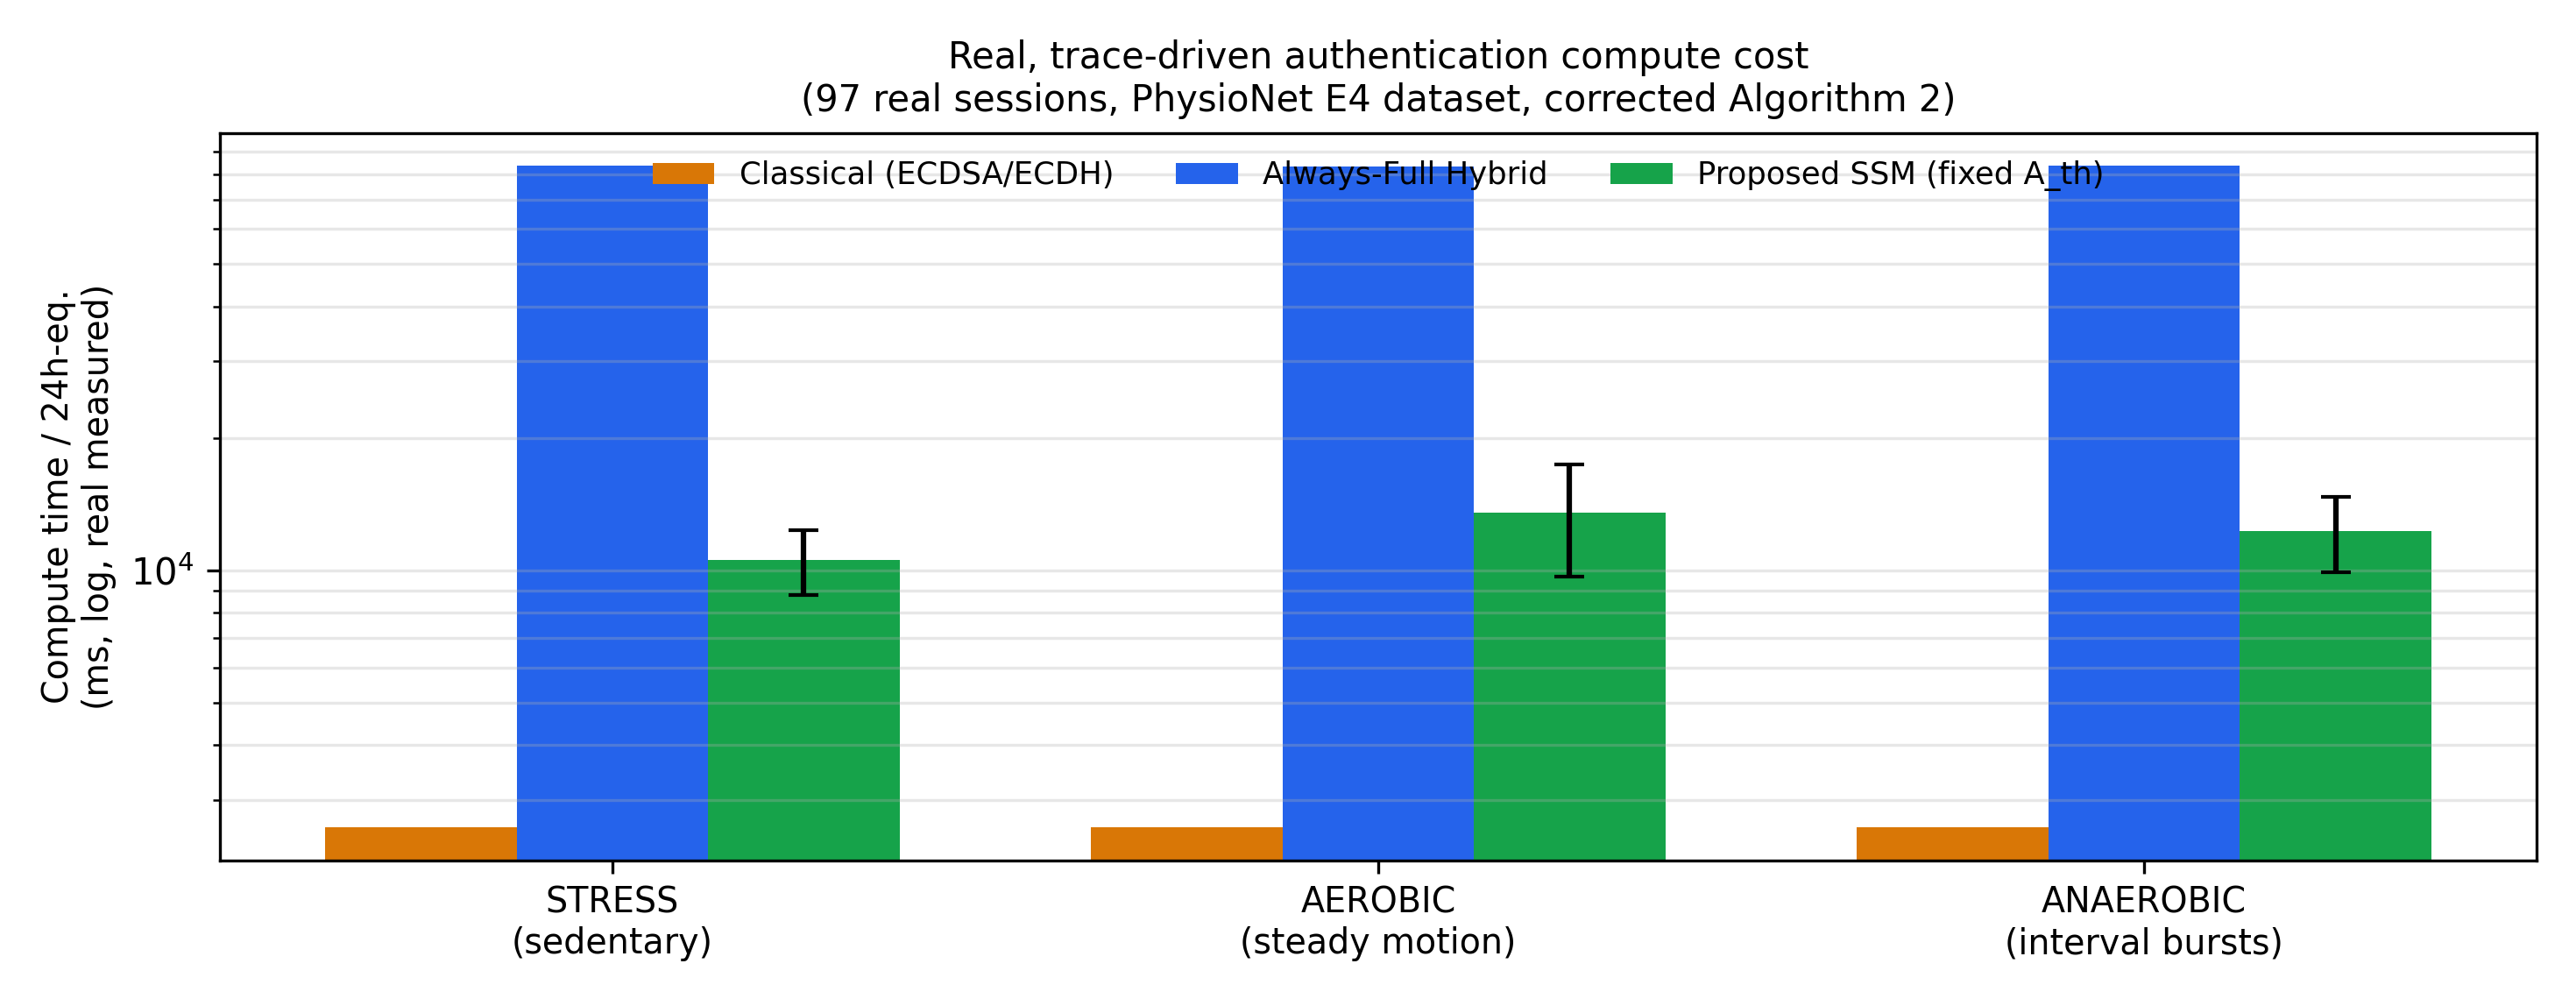
\includegraphics[width=\columnwidth]{../figures/fig3_compute_cost.png}
\caption{Real, trace-driven authentication compute cost (97 real sessions,
PhysioNet E4 dataset, corrected Algorithm 2). Log scale; error bars are
real cross-session standard deviation, not simulated variance.}
\label{fig:fig3}
\end{figure}

\textbf{Reproducibility note.} Bandwidth-reduction percentages are exact
and bit-for-bit reproducible on any machine, since they come from fixed
serialized message sizes. Compute-time-reduction percentages depend on a
real wall-clock crypto benchmark and carry roughly $\pm0.5$ percentage
point run-to-run variance (observed directly across two clean pipeline
runs in this work); a reader re-running the accompanying \texttt{run\_all.py}
on their own machine should expect the figures above to within this
margin, not bit-for-bit.

\subsection{Threshold Sensitivity}

Because $T_{max}$, $R_{max}$ and $A_{th}$ are configurable design
parameters, we re-ran the same trace-driven methodology on the AEROBIC
regime while varying each parameter in turn, holding the other two at
their frozen defaults (Fig.~\ref{fig:fig4}, Fig.~\ref{fig:fig5}) -- a real
re-execution of Algorithm~1 over the same real data for every point
plotted, not an assumed curve.

\begin{figure}[t]
\centering
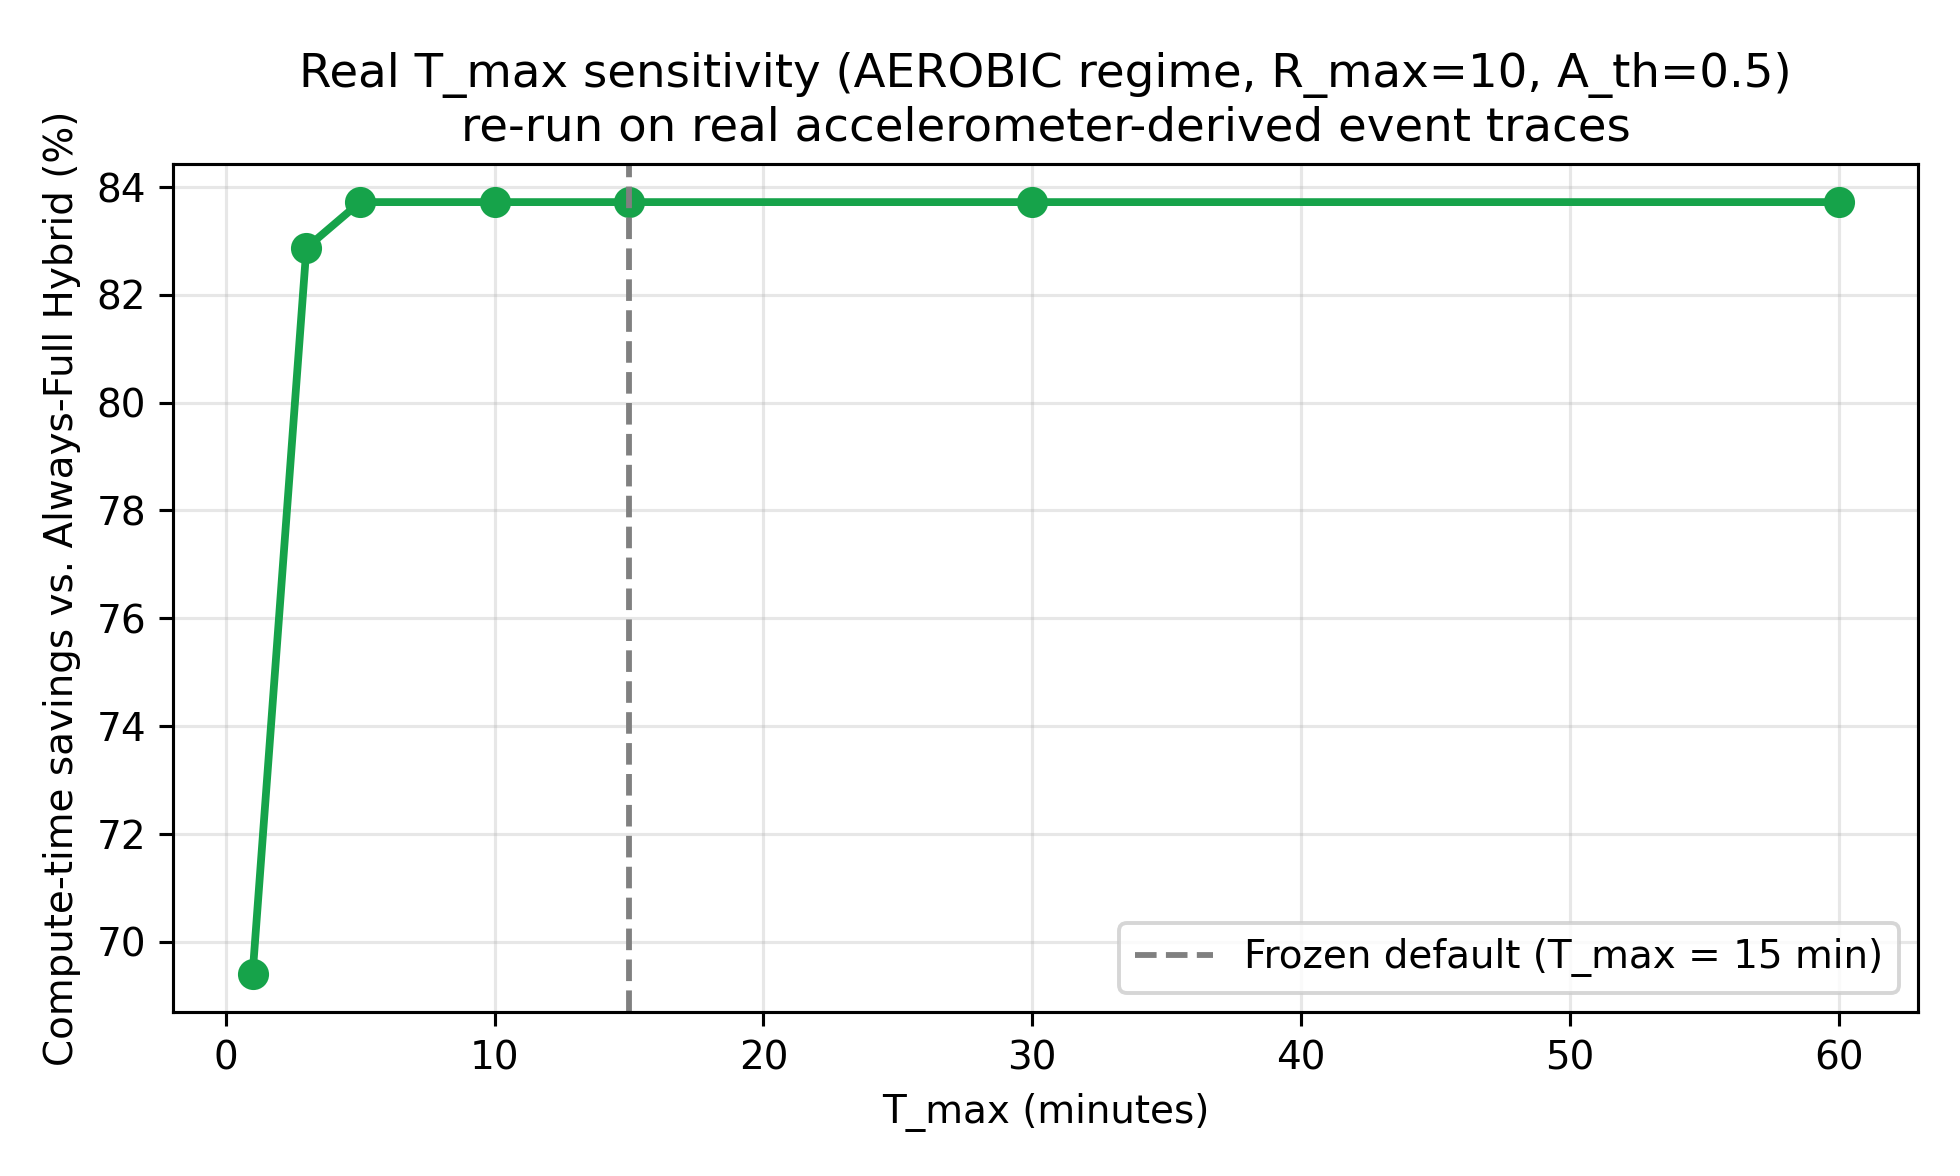
\includegraphics[width=\columnwidth]{../figures/fig4_sensitivity_tmax.png}
\caption{Real $T_{max}$ sensitivity (AEROBIC regime, $R_{max}=10$,
$A_{th}=0.5$), re-run on real accelerometer-derived event traces.}
\label{fig:fig4}
\end{figure}

\begin{figure}[t]
\centering
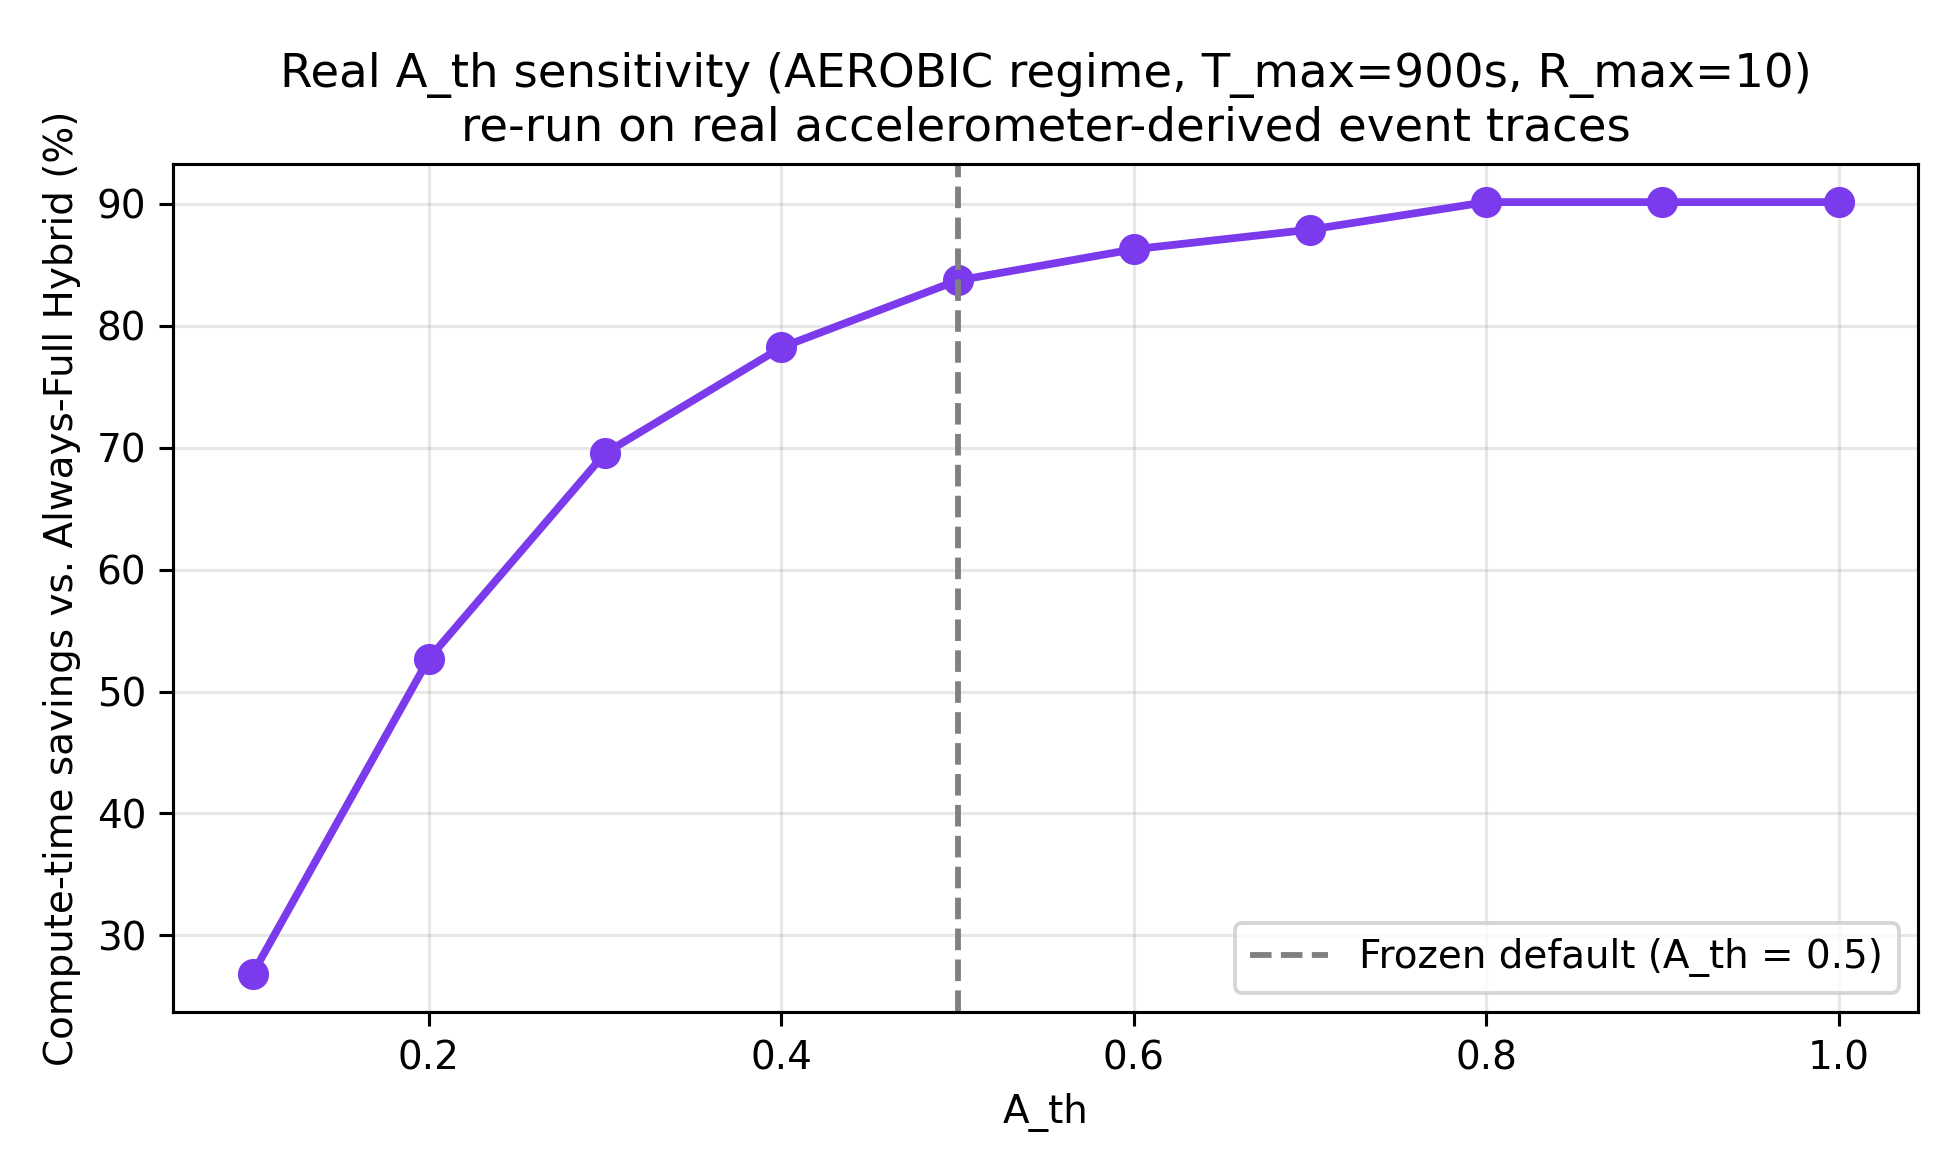
\includegraphics[width=\columnwidth]{../figures/fig5_sensitivity_ath.png}
\caption{Real $A_{th}$ sensitivity (AEROBIC regime, $T_{max}=900$~s,
$R_{max}=10$), re-run on real accelerometer-derived event traces.}
\label{fig:fig5}
\end{figure}

Real measured savings rise from 69.4\% at $T_{max}=1$~min and plateau at
83.7\% from $T_{max}\approx5$~min onward through $T_{max}=60$~min. As with
the earlier version of this design, at a 20-second check cadence
$R_{max}=10$ bounds any resumption chain to 200 seconds once $T_{max}$
exceeds that bound, so $R_{max}$ remains an equally important tuning
target as $T_{max}$ under this configuration -- this structural conclusion
is unchanged by the $A_{th}$ correction, since it follows from the
elapsed-time and count checks (Algorithm~1, lines~3--4), not the anomaly
branch. Unlike the earlier, mathematically-unreachable $A_{th}=1.5$
setting, sweeping $A_{th}$ now shows a real, monotonic effect on savings
(26.8\% at $A_{th}=0.1$ rising to a 90.1\% plateau from $A_{th}\approx0.8$),
confirming that the anomaly branch is now mechanically live rather than
dead code, and that $A_{th}=0.5$ sits at a real, non-edge point on this
curve rather than an extreme.

\subsection{Sanity Trace}
\label{sec:sanity}

For direct comparability with prior iterations of this work, we retain a
25-event trace over subject S01/AEROBIC's first 25 real reconnection
windows, run through the same \texttt{ssm\_engine.py} used everywhere else
in this paper. We label this explicitly a \emph{sanity/reproducibility
trace}, not a real-world evaluation claim, since 25 events from one subject
is illustrative rather than representative. With the corrected
$A_{th}=0.5$, this trace now produces 4 full authentications and 21
resumptions (5{,}728 bytes total), genuinely different from any prior
iteration's illustrative trace, because the anomaly branch can now actually
fire within this window -- exactly the expected consequence of the
$A_{th}$ correction (Sec.~\ref{sec:alg2}), not a discrepancy to reconcile.

\section{Discussion}

\subsection{Comparison with an Earlier Iteration of this Work}
\label{sec:audit}

An earlier iteration of this framework reported 74.5--85.0\% compute-time
reduction and 67.0--76.4\% bandwidth reduction. This project's own
reproducibility audit of that earlier iteration
(\texttt{paper/audit/OLD\_PAPER\_AUDIT.md}) found that those figures were
generated by a scoring path that compared a raw z-score directly against
$A_{th}$, bypassing Algorithm~2's clamped formula entirely, and used a
per-file session count that double-counted the three split-recording
subjects (Sec.~\ref{sec:eval-a}). The results in Sec.~\ref{sec:results} are
produced by the corrected algorithm, the corrected session count, and the
frozen split/duplication decisions of Sec.~\ref{sec:eval-a}, none of which
were tuned toward or away from the earlier iteration's numbers or toward
any other previously-computed estimate; the full side-by-side comparison,
including which methodological differences are believed to explain the
change, is in the supplementary \texttt{OLD\_VS\_NEW\_AUDIT.md}. We report
this comparison for transparency about how this line of work has evolved,
not as validation that either number is more ``correct'' in isolation --
each is what its own methodology produces.

\subsection{Practical Deployment}

The framework reduces authentication overhead by avoiding unnecessary
cryptographic operations while maintaining quantum-resistant guarantees,
and degrades gracefully to a conventional hybrid handshake if resumption is
disabled. It still depends on secure gateway infrastructure to host the SSM
and ticket store, and on trusted device registration -- neither of which
the protocol itself secures. The bounded design trades a small increase in
protocol complexity and one additional stored secret ($K_r$) per device for
a substantial, quantified reduction in per-session cost, favorable for
continuously connected, battery-constrained deployments but requiring
threshold configuration that a stateless always-full design does not.

\section{Limitations}
\label{sec:limits}

Performance figures for Ed25519, HMAC, AES-128-GCM and HKDF are measured
directly by the accompanying open-source reference implementation on a
commodity x86-64 CPU (software-only), not on embedded Cortex-M4 hardware;
absolute latencies would differ on target hardware, though the relative
full-vs-resumption structure is expected to hold. The ML-KEM-512
implementation used here is an unoptimized pure-Python reference
(\texttt{kyber-py}), not an embedded-optimized C/assembly implementation,
so its absolute cost -- and consequently the full handshake's cost
relative to classical ECDSA/ECDH -- is inflated relative to what optimized
embedded PQC libraries report; we do not claim ML-KEM is intrinsically more
or less expensive than ECDH from this measurement alone. Compute-time
reduction percentages carry roughly $\pm0.5$ percentage point run-to-run
timing variance from this real benchmark; bandwidth reduction is exact.
Reconnection-event timing and the anomaly-score feature are derived from
real accelerometer telemetry of a real BLE wearable rather than assumed
distributions, but that dataset comprises structured 25--45 minute
laboratory sessions rather than continuous 24-hour real-world wear, so the
24h-equivalent figures in Table~\ref{tab:table3} are a disclosed linear
extrapolation of real per-session rates, not a genuine day-long recording.
$\mathit{failed\_resumptions}$ is fixed at 0 throughout the real-dataset
experiment because the dataset contains no real authentication-failure
signal, so this term of Algorithm~2 is untested against real failure data.
HR/IBI signal ambiguity for subject S02/STRESS (Sec.~\ref{sec:eval-a}) is
unresolved; it does not affect this paper's results, which use only
accelerometer magnitude, but we state it rather than silently ignoring it.
$w_1$, $w_2$ and $A_{th}$ remain configuration parameters rather than
values fit to labeled attack data. The formal verification in
Sec.~\ref{sec:fv} covers a single protocol session in full; the
unbounded-session attempt produced one open, unresolved finding, most
likely a modeling gap rather than a real vulnerability, but not confirmed
as such. Side-channel resistance of the underlying Ed25519 and ML-KEM
implementations has not been independently assessed for this deployment.

\textbf{This paper makes no energy claim anywhere.} Only compute time (ms)
and bytes are measured and reported.

\section{Conclusion}

This paper presented an adaptive hybrid authentication framework for
wearable healthcare systems, centered on a Session Security Manager that
decides, per reconnection, between a full Ed25519 identity-verification +
ML-KEM-512 quantum-resistant key-establishment handshake and a bounded,
quantum-safe-rooted lightweight resumption -- backed by a formalized
anomaly-scoring algorithm whose threshold is corrected to be mathematically
reachable within the score's own declared range, a fix pre-registered
before the experiment that produced this paper's results. A fully
reproducible, trace-driven evaluation -- combining a real, benchmarked
cryptographic reference implementation with real accelerometer telemetry
and three documented real Bluetooth-disconnection incidents from a public
wearable-device dataset, under an explicit, pre-registered methodology for
split recordings and a documented signal duplication -- showed compute-time
reductions of 83.7--87.3\% and bandwidth reductions of 75.3--78.6\% versus
an always-full hybrid baseline, without asserting energy figures. Real,
distinctly different results from an earlier iteration of this work confirm
that the correction changes the algorithm's actual behavior rather than
merely its stated threshold. Single-session formal verification in
ProVerif found all eight secrecy and injective-correspondence queries true
after correcting a backwards-direction specification bug from an earlier
model; an unbounded verification attempt is reported honestly as producing
one open, unresolved finding rather than a claimed pass. Comparison against
recent hybrid PQC healthcare-IoT proposals suggests that, to the best of our
knowledge, this adaptive-resumption gap is not addressed elsewhere in the
surveyed literature. Immediate next steps are to resolve the unbounded
verification finding with an explicit shared-counter model, port the
reference implementation to constrained hardware such as an ESP32 or nRF52
for direct embedded measurement, and gather a larger real incident sample
to properly fit Algorithm~2's anomaly-scoring weights.

\section*{Data and Code Availability}

The complete source code, the dataset download/verification script, the
processed feature table, all test suites, the ProVerif models and their raw
output, and the scripts that generate every table and figure in this paper
directly from measured results are available in the supplementary material
accompanying this submission (\texttt{run\_all.py} reproduces the entire
pipeline end to end). The raw PhysioNet dataset itself is not redistributed
due to its size and to keep the official PhysioNet download/verification
path authoritative; \texttt{src/preprocessing/download\_dataset.py}
reproduces it from the official source with SHA-256 verification against
PhysioNet's own checksums.

\begin{thebibliography}{00}
\bibitem{fips203} NIST, ``Module-Lattice-Based Key-Encapsulation Mechanism Standard (ML-KEM),'' FIPS PUB 203, 2024.
\bibitem{shor1994} P. W. Shor, ``Algorithms for quantum computation,'' in \emph{Proc. FOCS}, 1994, pp. 124--134.
\bibitem{gcm} NIST, \emph{Recommendation for Block Cipher Modes of Operation: GCM/GMAC}, SP 800-38D, 2007.
\bibitem{eddsa} S. Josefsson and I. Liusvaara, \emph{EdDSA}, RFC 8032, IETF, 2017.
\bibitem{hkdf} H. Krawczyk and P. Eronen, \emph{HKDF}, RFC 5869, IETF, 2010.
\bibitem{blanchet2016} B. Blanchet, ``Verifying security protocols with ProVerif,'' \emph{Foundations and Trends in Privacy and Security}, vol. 1, 2016.
\bibitem{cortexm4} K. Owens \emph{et al.}, ``Efficient, side-channel resistant Ed25519 on Cortex-M4,'' IEEE, 2024.
\bibitem{saarinen2020} M.-J. Saarinen, ``Mobile energy requirements of the post-quantum cryptography NIST candidates,'' arXiv:1912.00916, 2020.
\bibitem{pqm4} M. Kannwischer \emph{et al.}, ``pqm4: Benchmarking NIST PQC on Cortex-M4,'' Cryptology ePrint Archive, 2019/844.
\bibitem{wolfssl2024} wolfSSL, ``Post-Quantum Kyber Benchmarks,'' 2024.
\bibitem{kyber2018} J. Bos \emph{et al.}, ``CRYSTALS--Kyber: A CCA-secure module-lattice-based KEM,'' in \emph{Proc. IEEE EuroS\&P}, 2018.
\bibitem{abood2025} E. W. Abood, A. A. Yassin, Z. A. Abduljabbar, V. O. Nyangaresi, and A. H. Ali, ``Provably lightweight and secure IoHT scheme with post-quantum cryptography and fog computing,'' \emph{MethodsX}, 2025.
\bibitem{adeli2023} M. Adeli, N. Bagheri, H. R. Maimani, S. Kumari, and J. J. P. C. Rodrigues, ``A post-quantum compliant authentication scheme for IoT healthcare systems,'' \emph{IEEE Internet of Things Journal}, 2023.
\bibitem{alsaggaf2022} M. A. Al-Saggaf \emph{et al.}, ``Lightweight two-factor-based user authentication protocol for IoT-enabled healthcare ecosystem in quantum computing,'' \emph{Arabian J. Sci. Eng.}, 2022.
\bibitem{yan2026} H. Yan, Z. Wang, L. Lin, J. Sun, and S. Liu, ``A Kyber-based lightweight cloud-assisted authentication scheme for medical IoT,'' \emph{Sensors}, vol. 26, no. 7, 2026.
\bibitem{ferrag2021} M. A. Ferrag \emph{et al.}, ``Authentication protocols for Internet of Medical Things: A survey,'' \emph{IEEE Communications Surveys \& Tutorials}, vol. 23, 2021.
\bibitem{physionet-wearable} A. Hongn, F. Bosch, L. Prado, and P. Bonomini, ``Wearable Device Dataset from Induced Stress and Structured Exercise Sessions'' (version 1.0.0), PhysioNet, 2025, doi:10.13026/zzf8-xv61.
\bibitem{physionet} A. L. Goldberger \emph{et al.}, ``PhysioBank, PhysioToolkit, and PhysioNet: Components of a new research resource for complex physiologic signals,'' \emph{Circulation}, vol. 101, no. 23, pp. e215--e220, 2000.
\end{thebibliography}

\end{document}
